\inputencoding{utf8}

\lstset{
    breaklines=true,
    frame=single,
    keepspaces=true,
    numbers=left,
    moredelim = [s][\color{purple}]{/*}{*/},
    inputencoding = utf8,  % Input encoding
    extendedchars = true,  % Extended ASCII
    literate      =        % Support additional characters
      {á}{{\'a}}1  {é}{{\'e}}1  {í}{{\'i}}1 {ó}{{\'o}}1  {ú}{{\'u}}1
      {Á}{{\'A}}1  {É}{{\'E}}1  {Í}{{\'I}}1 {Ó}{{\'O}}1  {Ú}{{\'U}}1
      {à}{{\`a}}1  {è}{{\`e}}1  {ì}{{\`i}}1 {ò}{{\`o}}1  {ù}{{\`u}}1
      {À}{{\`A}}1  {È}{{\'E}}1  {Ì}{{\`I}}1 {Ò}{{\`O}}1  {Ù}{{\`U}}1
      {ä}{{\"a}}1  {ë}{{\"e}}1  {ï}{{\"i}}1 {ö}{{\"o}}1  {ü}{{\"u}}1
      {Ä}{{\"A}}1  {Ë}{{\"E}}1  {Ï}{{\"I}}1 {Ö}{{\"O}}1  {Ü}{{\"U}}1
      {â}{{\^a}}1  {ê}{{\^e}}1  {î}{{\^i}}1 {ô}{{\^o}}1  {û}{{\^u}}1
      {Â}{{\^A}}1  {Ê}{{\^E}}1  {Î}{{\^I}}1 {Ô}{{\^O}}1  {Û}{{\^U}}1
      {œ}{{\oe}}1  {Œ}{{\OE}}1  {æ}{{\ae}}1 {Æ}{{\AE}}1  {ß}{{\ss}}1
      {ç}{{\c c}}1 {Ç}{{\c C}}1 {ø}{{\o}}1  {Ø}{{\O}}1   {å}{{\r a}}1
      {Å}{{\r A}}1 {ã}{{\~a}}1  {õ}{{\~o}}1 {Ã}{{\~A}}1  {Õ}{{\~O}}1
      {ñ}{{\~n}}1  {Ñ}{{\~N}}1  {¿}{{?`}}1  {¡}{{!`}}1
      {°}{{\textdegree}}1 {º}{{\textordmasculine}}1 {ª}{{\textordfeminine}}1
      % ¿ and ¡ are not correctly displayed if inconsolata font is used
      % together with the lstlisting environment. Consider typing code in
      % external files and using \lstinputlisting to display them instead.
  }


\section{Etape 1 : Modéliser, définir le problème formel, associer une classe de complexité}

  \subsection{Question 1 : Modélisation et caractéristiques}

    Les problèmes formels soulevés seront développés dans la deuxième question.

    Voici les propriétés du premier graphe que nous avons trouvé en étudiant le problème :

    \begin{itemize}
     \item Non orienté
     \item Non complet
     \item Trois types de noeuds différents mais les intersections de rues ou de métro ont le même comportement.
    \end{itemize}


    \begin{figure}
            \centering
                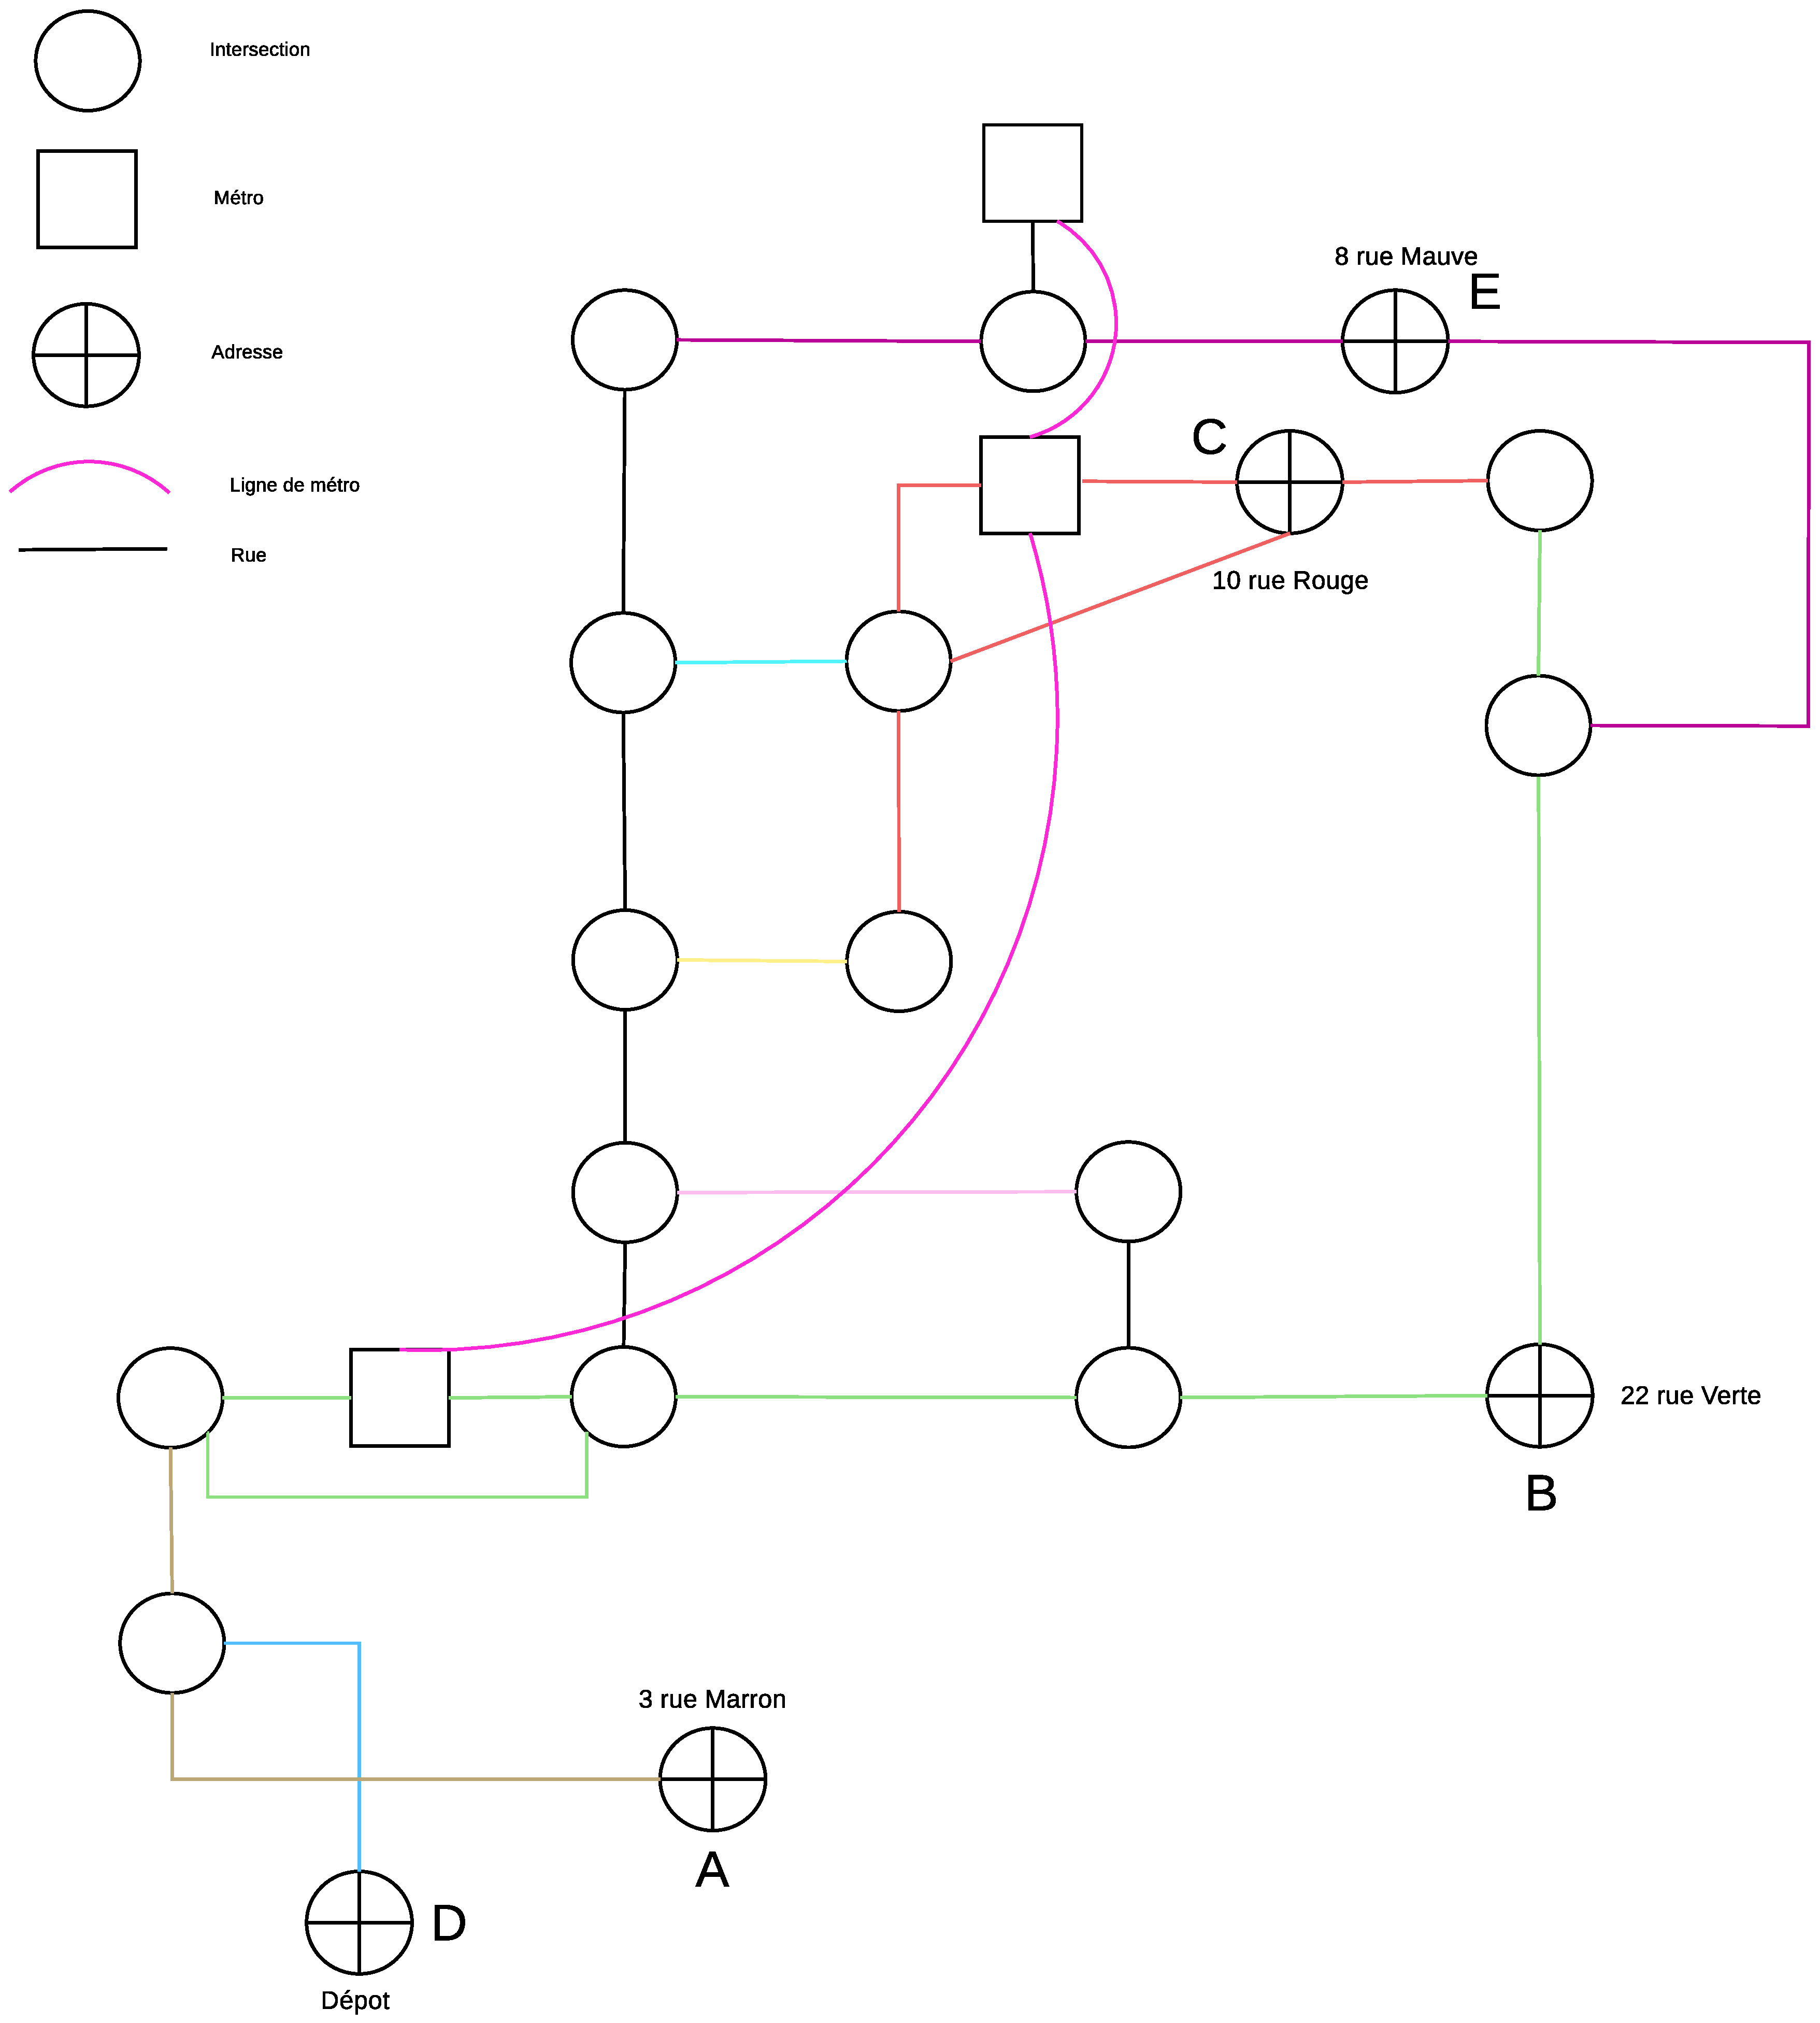
\includegraphics[width=0.8\textwidth]{images/graphe.eps}
            \caption{Représentation sous forme de graphe du problème}
            \label{fig:graphe} % Étiquette pour y faire référence ailleurs dans le document
    \end{figure}

    \newpage

    Le deuxième graphe a été créé à partir du premier, en voici les propriétés :

    \begin{itemize}
     \item Non orienté
     \item Complet
     \item Un noeud symbolise une adresse
     \item Une arête est le chemin le plus court entre deux adresses
    \end{itemize}


    \begin{figure}[h!]
            \centering
                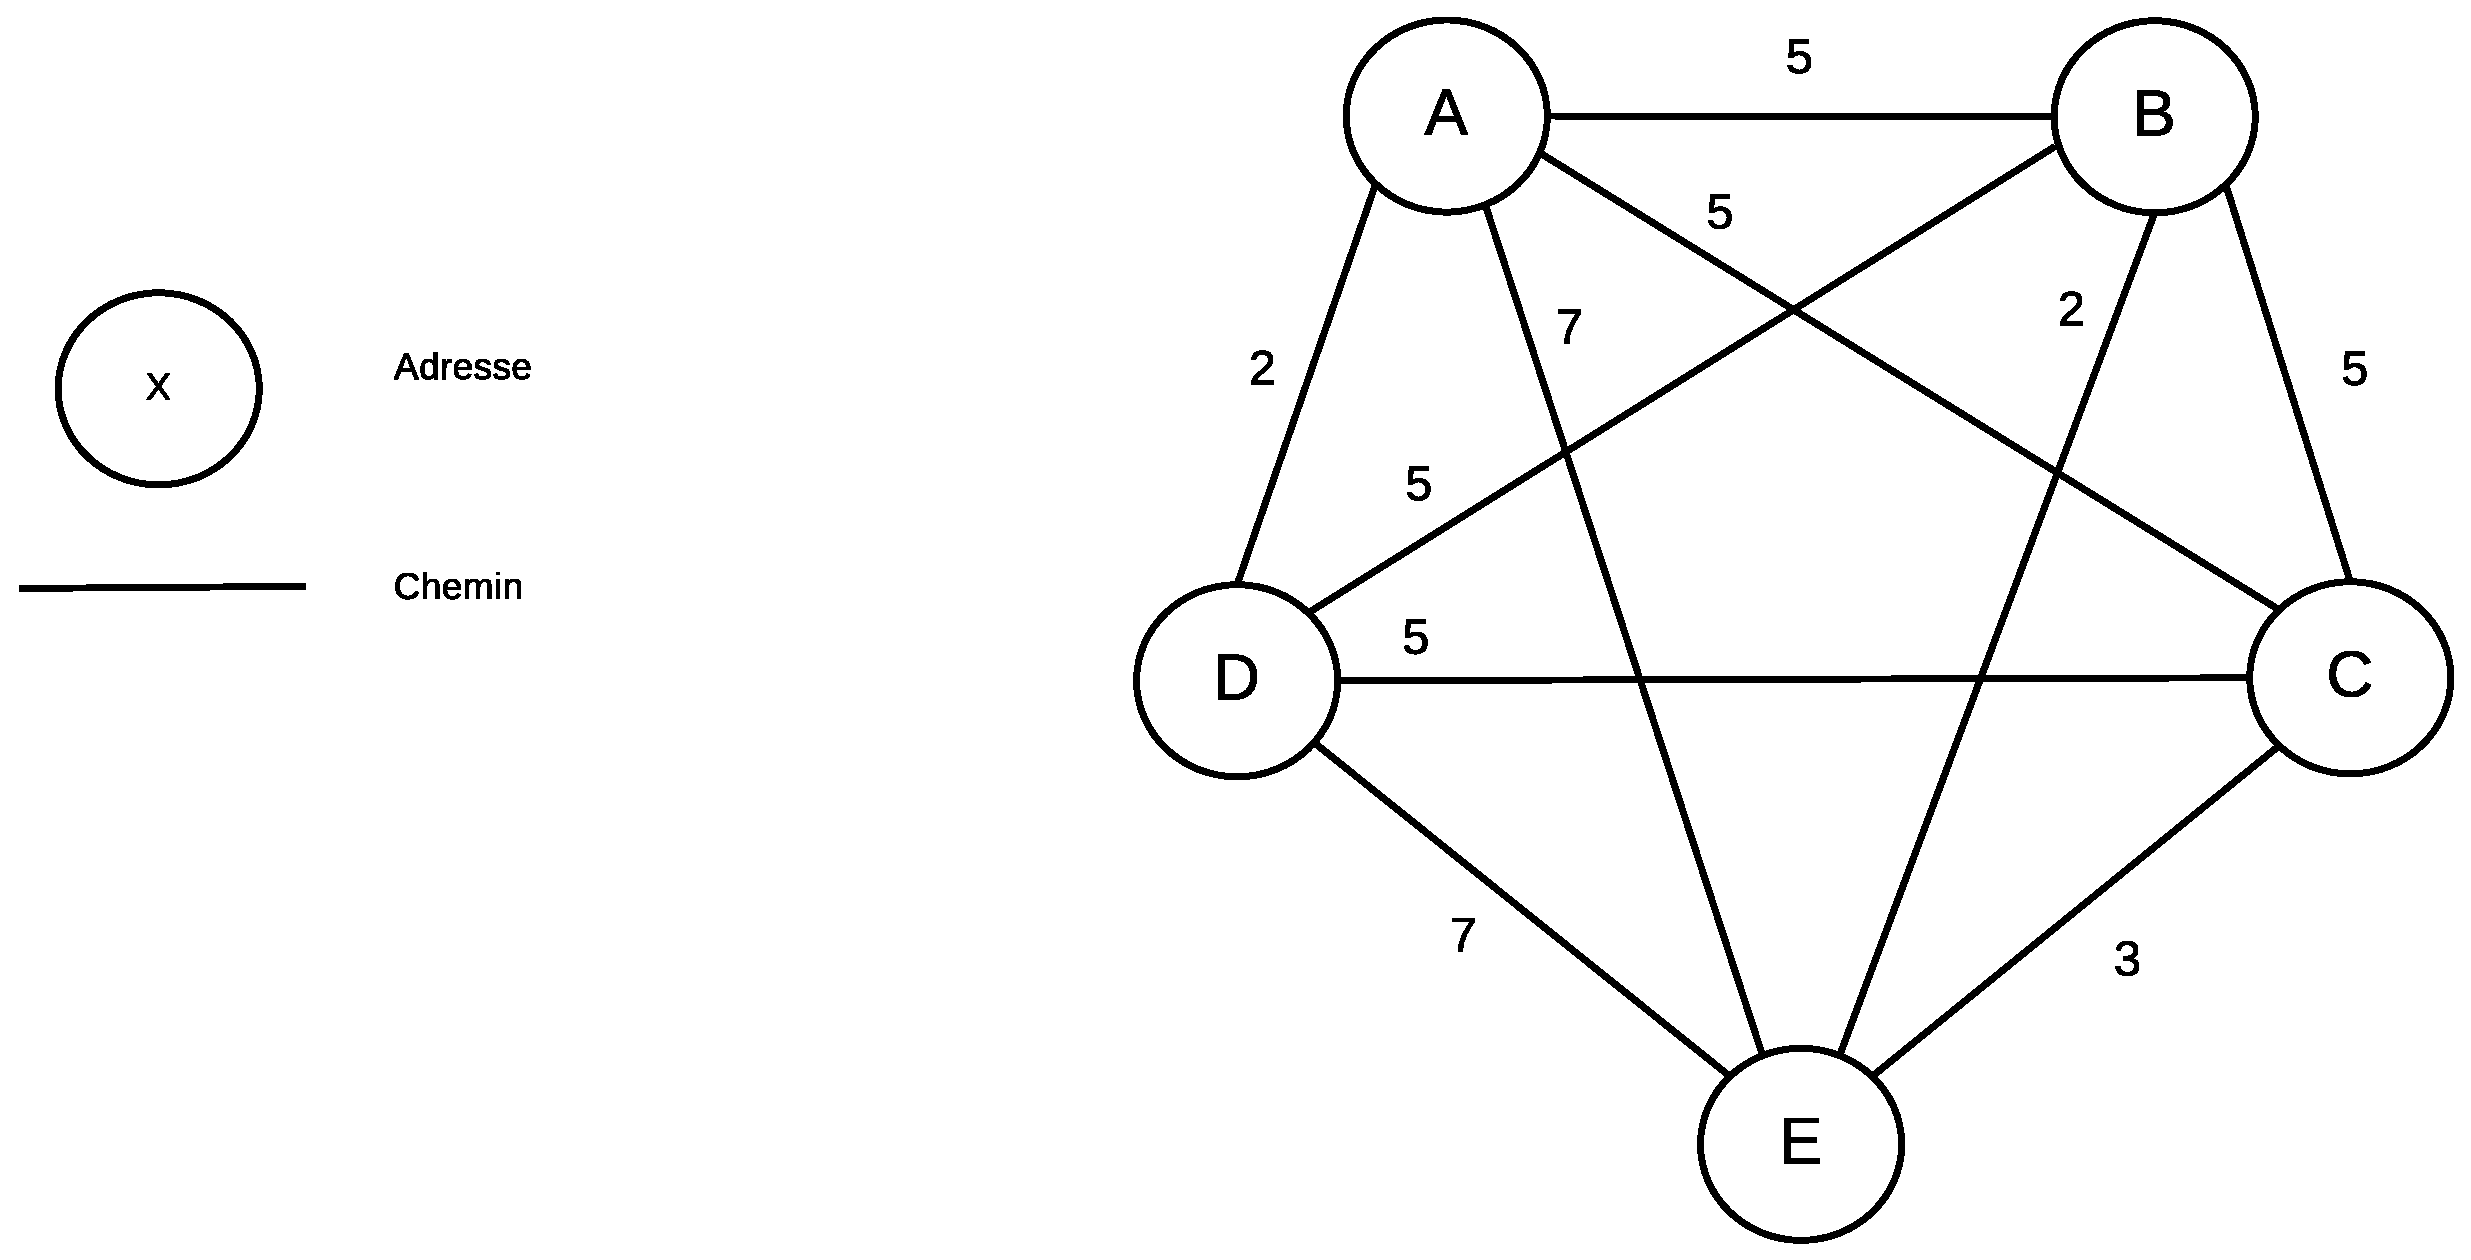
\includegraphics[width=1\textwidth]{images/graphe2.eps}
            \caption{Représentation sous forme de graphe du deuxième problème}
            \label{fig:graphe} % Étiquette pour y faire référence ailleurs dans le document
    \end{figure}

    \clearpage


  \subsection{Question 2 : Problèmes formels}
    Le problème est celui du voyageur de commerce. En effet, il faut trouver un cycle hamiltonien qui passe par les adresses, mais il doit avoir un coût minimal.

    Actuellement, il faut prévoir deux types de noeud : intersection de rues et d'adresses, mais nous avons rajouté la distinction entre rue et métro à l'avance. On peut repasser plusieurs fois par une intersection de rue ou de métro, mais pas d'une adresse. De plus, si le métro est indisponible, il faut pouvoir le retirer facilement du graphe et n'utiliser que les intersections de rues. Il a été aussi décidé de matérialiser les adresses sous forme de noeuds, sinon impossible d'aller 3 rue marron et d'y revenir si cela avait été une arête. Il aurait fallu en plus matérialiser les fins de rues. Cela permet d'aller à une adresse et de rebrousser chemin si besoin.
    Les arêtes permettent de compter le coût de déplacement puisqu'emprunter une arête coûte 1.

    Un deuxième graphe a été créé à partir du premier. Il s'agit d'un graphe complet avec le coût pour aller d'une adresse à une autre, où chaque noeud est une adresse et chaque arête est le coût du plus court chemin.

  \subsection{Question 3 : Complexité}
    Le problème est un Problème d'Optimisation Combinatoire (POC). La complexité est non polynomiale et c'est un PE associé NP-complet.
    Pour un ensemble de n points, on a $\frac{(n-1)!}{2}$ possibilités, c'est donc une complexité factorielle en n.

    Nous avons 22 noeuds pour le problème étudié. Cependant, nous avons 5 adresses et nous en calculons les combinaisons grâce au graphe 2. Nous obtenons 12 chemins possibles. Il est donc aisé de comparer et de trouver le chemin idéal. Si, à contrario, nous avions le double d'adresses, nous aurions une complexité de 2520, ce qui montre la croissance exponentielle de ce type de problème.

    \newpage


\section{Etape 2 : L'algorithme}

  \subsection{Question 1 : Etat de l'art et sources}
    \paragraph{Etat de l'art}
    \begin{itemize}
     \item \href{https://fr.wikipedia.org/wiki/Probl%C3%A8me_du_voyageur_de_commerce#:~:text=En%20informatique,%20le%20probl%C3%A8me%20du,une%20et%20une%20seule%20fois.}{Problème du voyageur de commerce - Wikipedia}
     \item \url{https://interstices.info/le-probleme-du-voyageur-de-commerce/}
     \item \url{https://math.unice.fr/~pauly/Little.pdf}
    \end{itemize}

    \paragraph{Algorithmes}
    \begin{itemize}
     \item \url{https://rosettacode.org/wiki/Dijkstra's_algorithm#C}
     \item \url{https://www.programiz.com/dsa/dijkstra-algorithm}
     \item \url{https://en.wikipedia.org/wiki/Branch_and_bound}
     \item \url{https://www.jot.fm/issues/issue_2005_01/article5.pdf}
    \end{itemize}

  \subsection{Question 2 : Pseudo code}
      \subsubsection{Pseudo Code général}
        \begin{lstlisting}
  g <- graphe du probleme
  adresses <- noeuds de g étant des adresses
  t <- nouveau graphe transformé à partir de Dijkstra

  Pour chaque a dans adresses
    dist, prev <- dijkstra(g, a)
    Pour chaque b dans adresses
      Si b != a et NON t.existeArc(a, b)
        t.ajouterArc(a, b, dist[b])

  meilleurChemin <- brute force sur t pour trouver le chemin hamiltonien le plus court




        \end{lstlisting}

        \newpage

      \subsubsection{Pseudo Code Brute force}
        \begin{lstlisting}
fonction bruteForceTSP(Graphe G, Sommet S): Liste de Sommet

  coutMini <- INFINI
  meilleurChemin <- Liste de sommet vide
  cheminsPossibles <- toutes les combinaisons de chemins possibles

  Pour chaque chemin dans cheminsPossibles Faire
    cout <- calcul du cout total du chemin
    Si cout < coutMini Alors
      coutMini <- cout
      meilleurChemin <- chemin

  Retourner meilleurChemin




        \end{lstlisting}

  \newpage

      \subsubsection{Pseudo Code Djikstra}
        \begin{lstlisting}
function dijkstra(G, S, metroEnPanne):

  P <- Liste de sommet vide   /*liste des noeuds déjà explorés*/
  Q <- Liste de sommet vide   /*liste des noeuds à explorer*/

  Pour chaque sommet V dans G
    distance[V] <- infini
    previous[V] <- NULL
    Si V != S Alors
      ajouter V à Q
  distance[S] <- 0


  Tant que Q est NON VIDE
    U <- noeud pas encore exploré le plus proche de S
    retirer U de Q
    ajouter U à P
    Pour chaque sommet V dans Q
      Si g.existeArc(U, V) Alors    /*Si V est voisin de U*/
        Si NON metroEnPanne OU V PAS de type [métro] Alors  /*Si le métro n'est pas en panne ou si le noeud n'est pas de type métro*/
          Si V PAS de type [adresse] OU V = S Alors   /*Si V n'est pas une adresse ou si V est le sommet de départ*/
            tempDistance <- distance[U] + g.valeurArc(U, V) /*On calcul la distance entre le voisin et U*/
            Si tempDistance < distance[V] Alors /*Si la distance est inférieur à la précédente on met à jour*/
              distance[V] <- tempDistance
              previous[V] <- U

  Retourner distance[], previous[]




        \end{lstlisting}


      \newpage


\section{Etape 3 : L'implémentation}

  \subsection{Le graphe utilisé par le programme}

    \begin{figure}[h!]
            \centering
                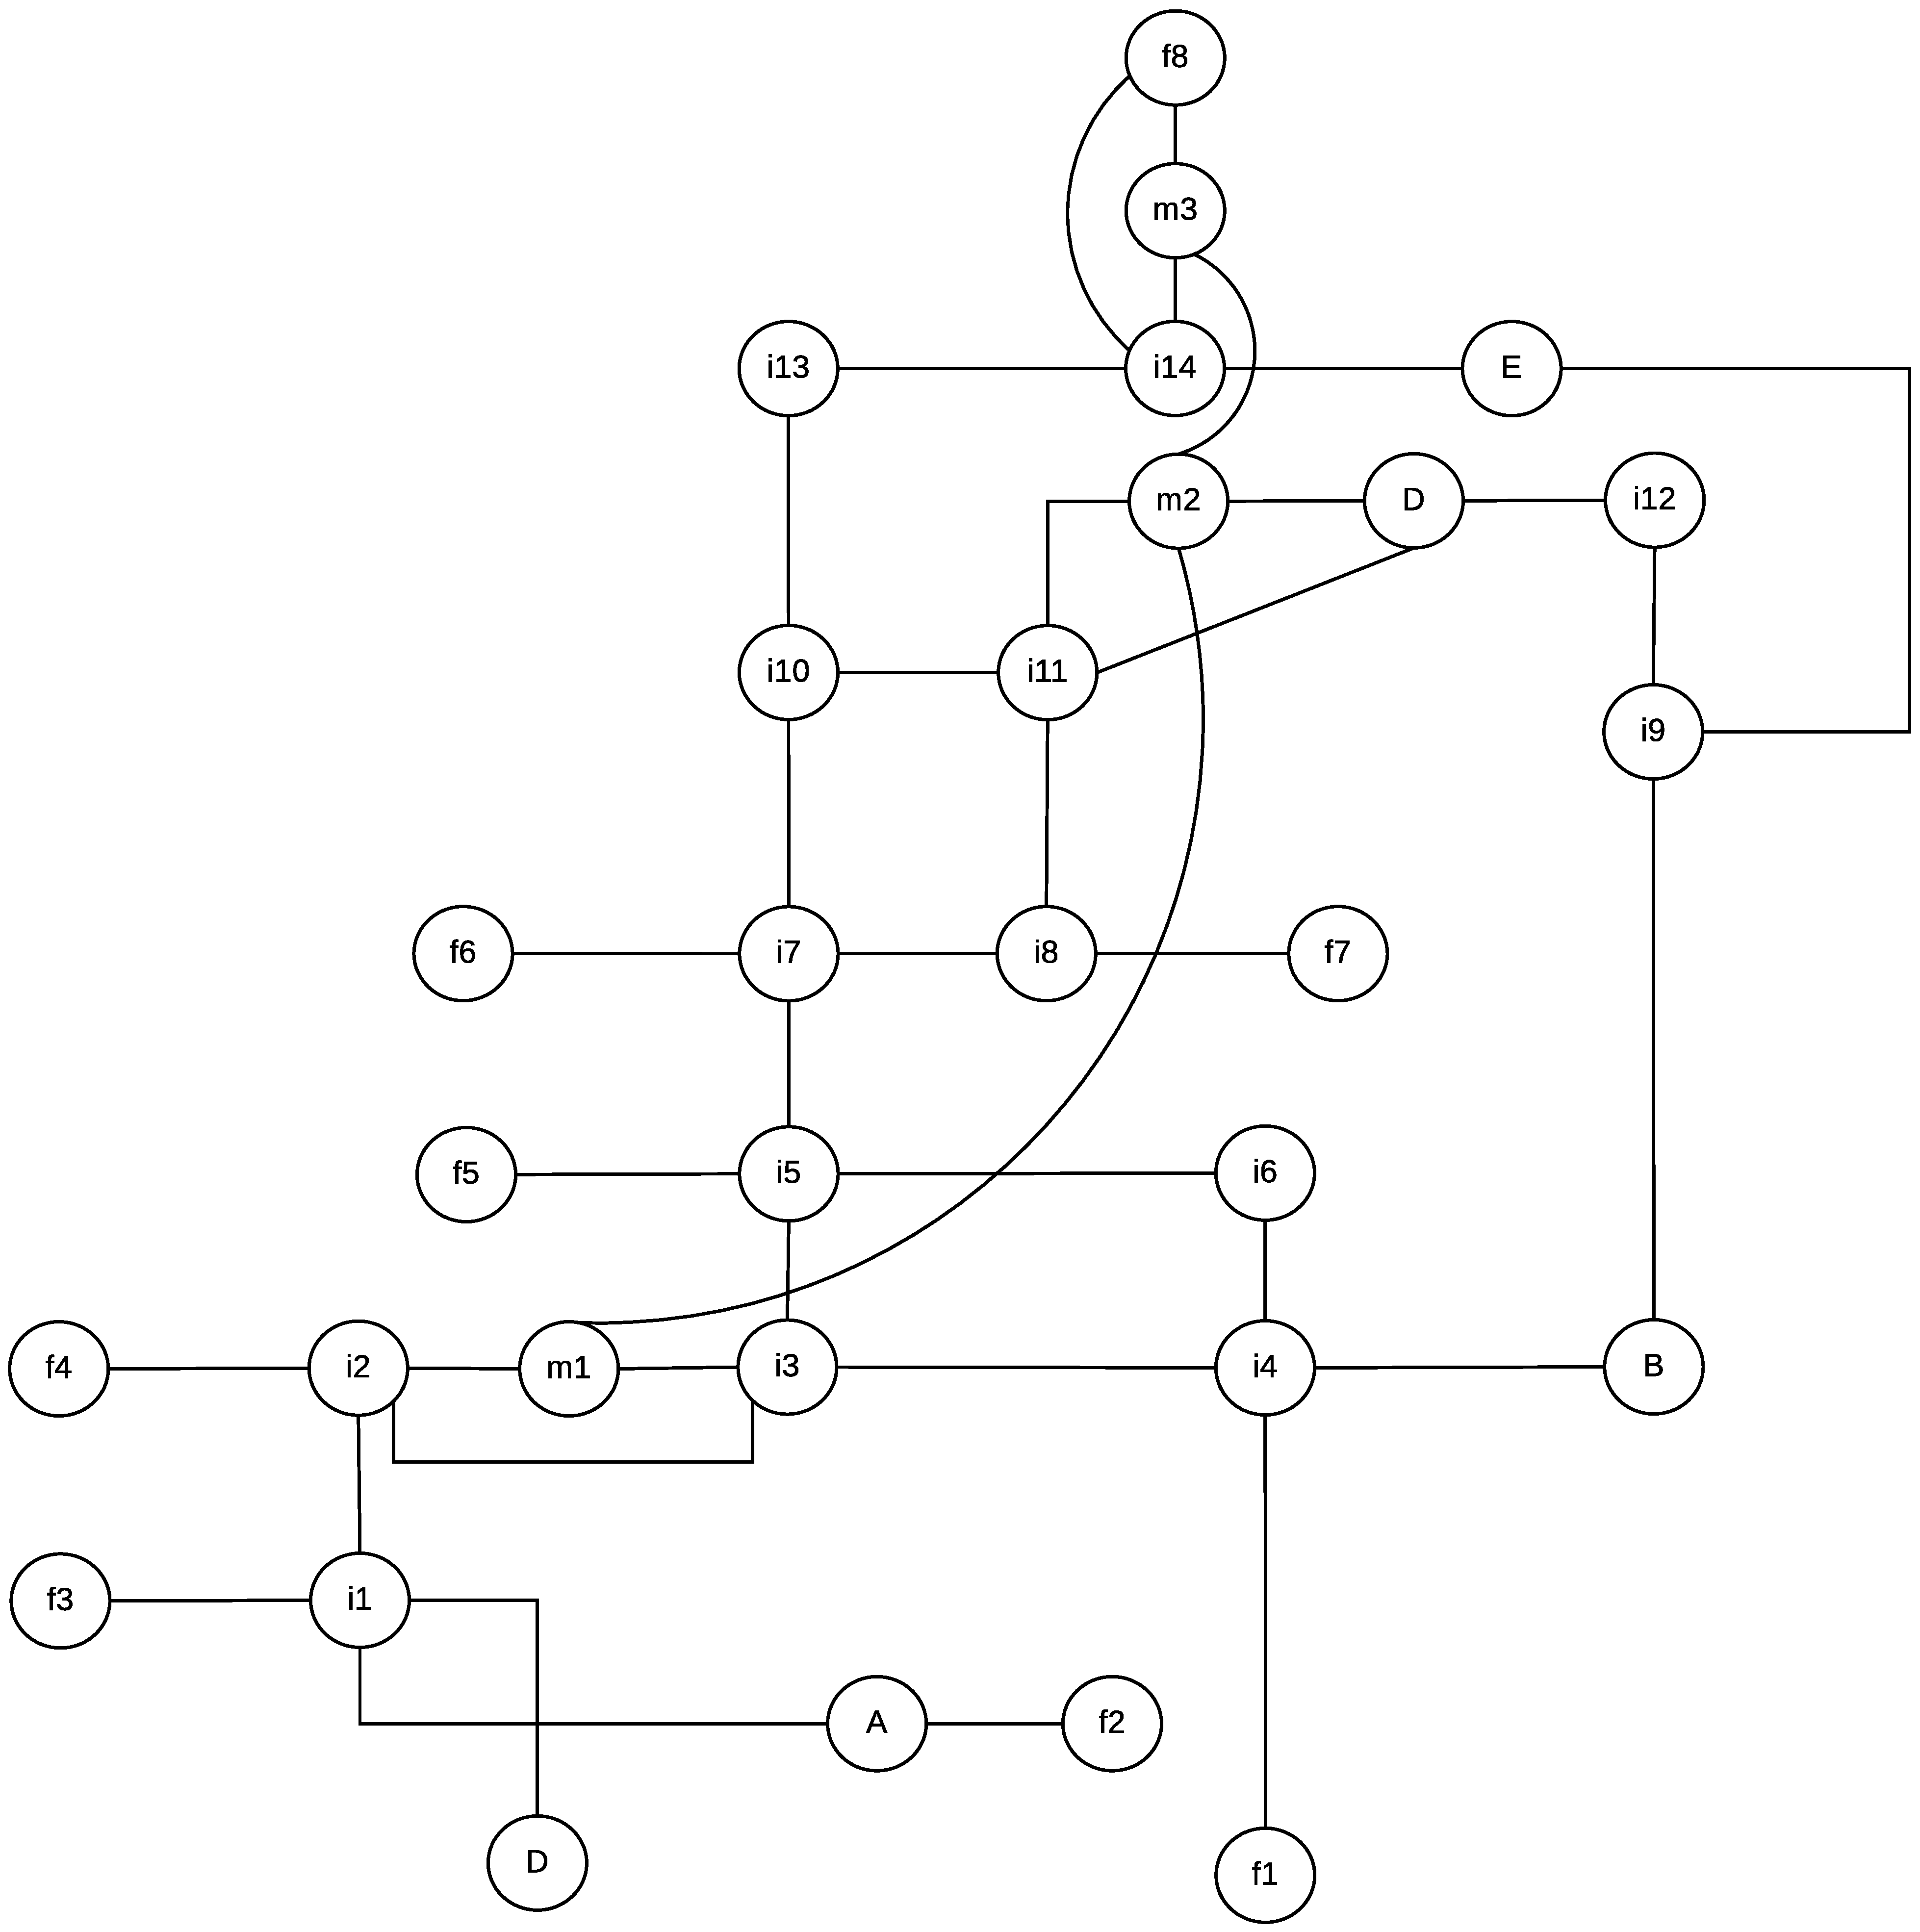
\includegraphics[width=0.9\textwidth]{images/grapheProgramme.eps}
            \caption{Représentation sous forme de graphe du problème que la machine interprête}
            \label{fig:graphe} % Étiquette pour y faire référence ailleurs dans le document
    \end{figure}

    \pagebreak


  \subsection{Le résultat}

    \begin{figure}[h!]
            \centering
                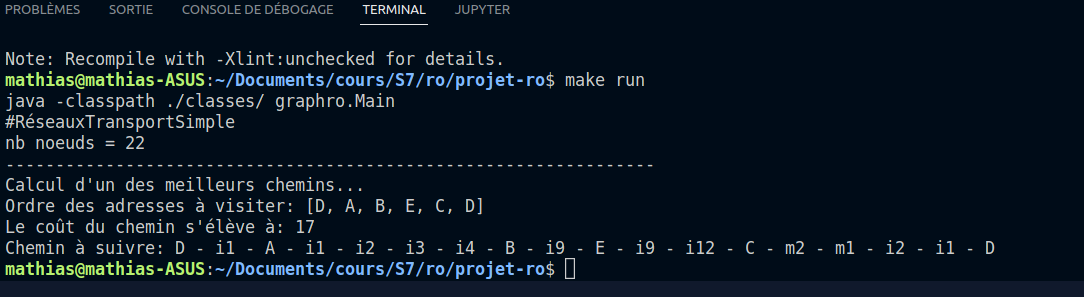
\includegraphics[width=1\textwidth]{images/resultatAvecMetro.png}
            \caption{Résultat du programme avec métro}
            \label{fig:graphe} % Étiquette pour y faire référence ailleurs dans le document
    \end{figure}

    \newpage



\section{Etape 4 : L'adaptation}

  \subsection{Question 1 : Métro en grève ?}
    Si le métro est en grève, il faut pouvoir retirer les noeuds correspondant au métro ainsi que les arêtes. C'est pour cette raison que nous les avons modélisés différemment.
  \subsection{Question 2 : Conséquences sur l'algorithme}
    Pour que l'algorithme prenne en compte cette variable, il suffit de différencier les noeuds à l'avance et grâce à une simple condition sur le type de noeud, on peut exclure le métro des combinaisons.
  \subsection{Question 3 : Implémentation}

    \begin{figure}[h!]
            \centering
                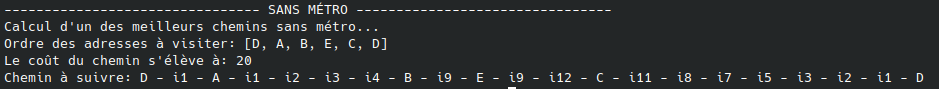
\includegraphics[width=1\textwidth]{images/resultatSansMetro.png}
            \caption{Résultat du programme sans métro}
            \label{fig:graphe} % Étiquette pour y faire référence ailleurs dans le document
    \end{figure}

    \newpage

